\documentclass{acm_proc_article-sp}
%\documentclass{IEEEtran}
%\usepackage[pdftex]{graphicx}

% correct bad hyphenation here
\hyphenation{op-tical net-works semi-conduc-tor}

\begin{document}

\title{URDAD as a Quality-Oriented Analysis and Design Process for Model Driven Development}

\numberofauthors{4}
\author{
\alignauthor
Fritz Solms\\
       \affaddr{Solms Training, Consulting and Development}\\
       \affaddr{113 Barry Hertzog Ave, Emmarentia, Johannesburg, 2915, South Africa}\\
       \email{fritz@solms.co.za}
\alignauthor
Riaan Klopper
       \affaddr{Dept. of Comp. Science, University of Pretoria, South Africa.}\\
		 \email{Riaan.Klopper2@standardbank.co.za}
\and
\alignauthor
Stefan Gruner\\
       \affaddr{Dept. of Comp. Science, University of Pretoria, South Africa.}\\
		 \email{sgruner@cs.up.ac.za}
\alignauthor
Derrick G. Koerie\\
       \affaddr{Dept. of Comp. Science, University of Pretoria, South Africa.}\\
		 \email{dkourie@cs.up.ac.za}
}


\maketitle


\begin{abstract}
The Use Case, Responsibility Driven Analysis and Design (URDAD) methodology, is
a methodology for technology neutral design generating the Platform Independent
Model (PIM) of the Object Management Group's (OMG's) Model Driven Architecture (MDA).
It requires the core modeling to be done in the problem space by
domain specialists and not in the solution space by technology specialists.
URDAD allows for formal elements to be
added by different role players at different stages of the model refinement,
whilst aiming to preserve agility of the outputs and low cost of the process
generating the outputs.
This paper discusses the semi-formal aspects of URDAD
which facilitate modeling validation and testing, documentation
generation and automated implementation mapping as well as aspects
which promote agility and low cost.
\end{abstract}

\keywords{ URDAD, model quality, model driven development, UML , MDA}

\section{Introduction}

The vision of model driven development (MDD)
\cite{schmidt:modelDrivenEngineering,stahl:mdsd}
even predates the definition of the Unified Modelling Language (UML); yet it
has historically been implemented with little success. With a cleaner separation of
architecture from design as envisaged by the Object Management Group's (OMG),
Model Driven Architecture (MDA) \cite{siegel:developingInMDA,frankel:enterpriseMDA}
together with semantically richer modelling languages like UML 2.x and stronger
tools support for MDD, the interest in MDD has increased considerably.

Yet there are a number of open issues which hold back the widespread adoption of MDD.
The first issue is the lack of a clear definition on what needs to be included in the
Platform Independent Model (PIM). Braek and Melby \cite{braek:modelDrivenServiceEngineering}
define a minimal requirements without specifying precisely the required components
for the PIM. This paper attempts to specify more concretely the artifacts which should
be included in a PIM.

The second issue is the lack of standards available to define the implementation architecture
and technologies required for the implementation mapping. This aspect is then often addressed in
a tool specific way like, for example, the cartridges approach of Andro-MDA. Usually this aspect
is further simplified by MDA tools supporting a specific set of reference architectures like
Java-EE, CORBA, CCM, JBI/SOA or Microsoft.Net.

The third issue slowing down the wide-spread adoption of MDA is the virtual lack of
a well defined, practical analysis and design methodology together with a
precise definition of the inputs and outputs
including the artifacts which must be included in the specification of a PIM.
which must be produced to define a required with specified inputs and outputs.

In this paper we will try and formulate some steps towards addressing the first
two issues. We will formulate some requirements for the PIM and will present
the Use-Case, Responsibility Driven Analysis and Design (URDAD)
\cite{solms:urdad}, a simple, algorithmic analysis and design methodology
which can be used by domain experts such as business analysts to generate the
PIM. The domain experts need not have an understanding of the implementation
architecture and technologies.

%--------------------------------------------------------------------

\subsection{Analysis and design methodologies}

Historically, URDAD has grown out of Responsibility Driven Design (RDD)
methodology pioneered by Rebecca Wirfs-Brock and Brian Wilkerson (see
\cite{wirfs-brock:responsibilityDrivenApproach},  and
\cite{wirfs-brock:objectDesign} \cite{wirfs-brock:designSimplicity}) and has
been influenced by the approaches of step-wise refinement \cite{wirth:stepWiseRefinement}
and top-down design \cite{martin:agileSoftwareDevelopment}.

But, while all of these are design approaches, URDAD provides an algorithmic
analysis and design methodology with the following characteristics:
\begin{enumerate}
  \item Both, requirements and design are step-wise refined.
  \item URDAD specifies the steps of the design methodology with
			well-defined inputs and outputs for each step, making the process repeatable
			and predictable.
  \item Generation of services contracts for the service providers required at any
			level of granularity enforcing a technology-neutral approach as well as
			pluggability and testability at any level of	granularity.
	\item Work flow logic at any level of granularity is factored out of the service
			providers for that level of granularity, enforcing decoupling of role players
			across levels of granularity.
	\item URDAD provides an explicit approach to fixing the levels of granularity.
   \item URDAD explicitly aims to generate a technology and architecture neutral design
			representing MDA's PIM.
\end{enumerate}

One of the benefits of having a standard design methodology generating a set of
predictable artifacts for the PIM, is that it simplifies the mapping from the platform
independent model (PIM) to the platform specific model (PSM), i.e.\ the methodology defines
standard set of source elements for the model transformations.

%------------------------------------------------------------------------------

\subsection{MDA-based development methodologies}

URDAD is usually embedded within an iterative realization or development process. Reviews of some
MDA-based development methodologies can be found in \cite{bercovici:businessArchitectureToSoa}
A typical model driven development process is shown in figure \ref{fig:developmentProcess}. 
Note that the technology neutral business process design is performed by business analysis. 
The technical team comprising both, architecture and implementation (development), 
is responsible for the realization of the business process within the chosen architecture and technologies.

\begin{figure}
  \centering
  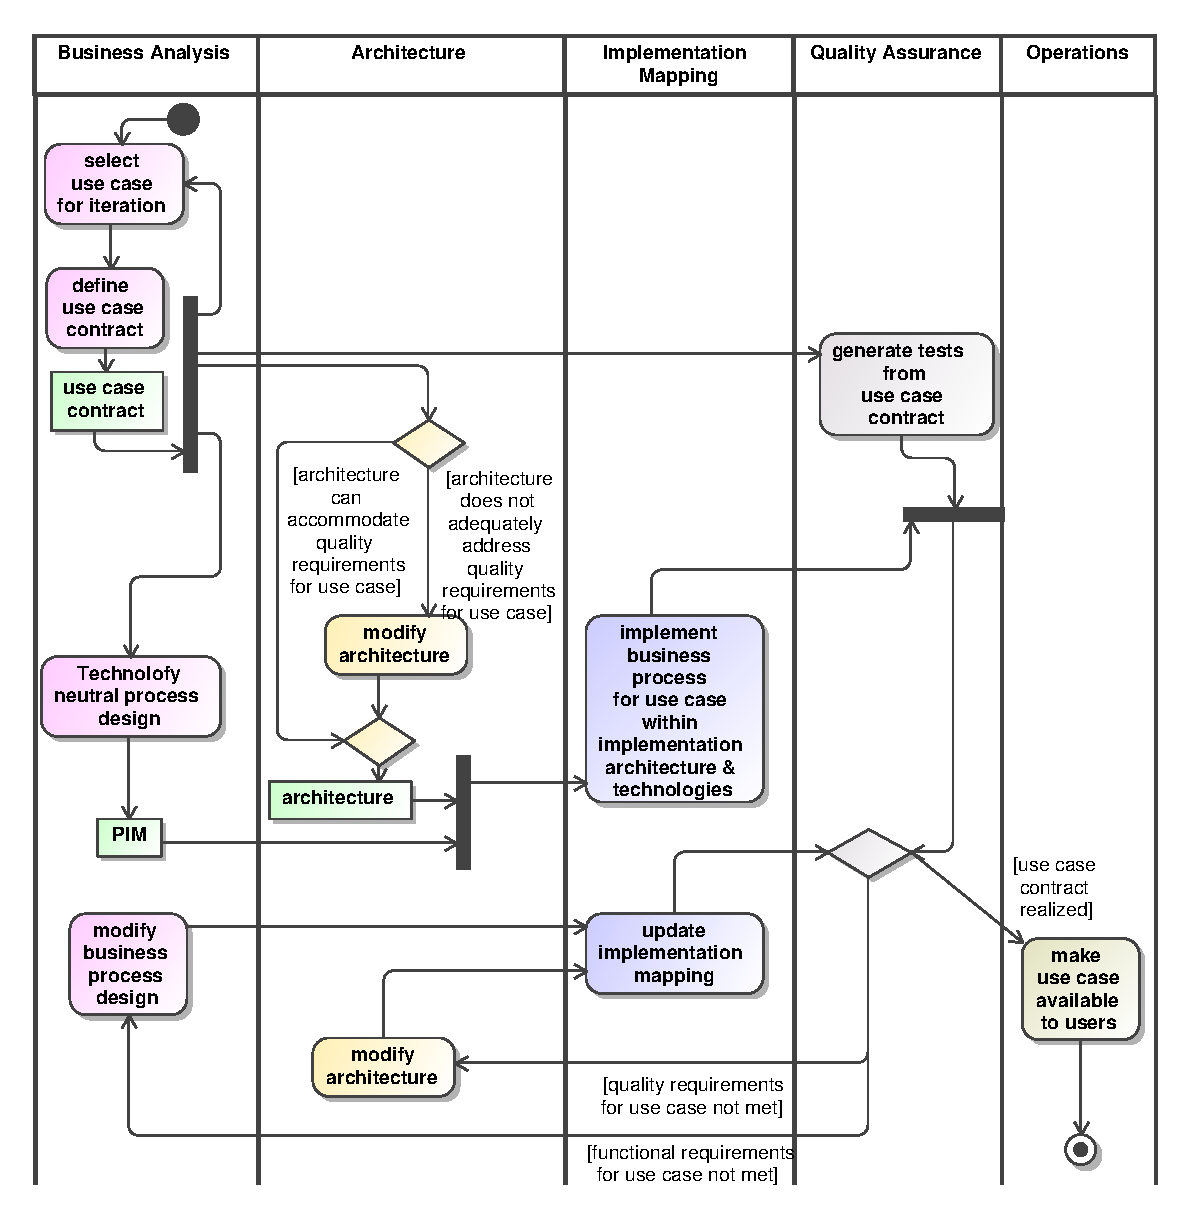
\epsfig{file=developmentProcess.eps, scale=0.6}
  \caption{Outline of a model driven development process.}
  \label{fig:developmentProcess}
\end{figure}

After passing quality assurance and actual deployment, operations takes over the management of the
business process execution.

%-------------------------------------------------------------------------------

\subsection{Real-life experiences with URDAD}

URDAD has been developed and taught to both business analysts and software designers since 2002.
More than a dozen of companies have been and are using URDAD for their technology neutral analysis
and design methodology. Some of these have decided to enforce the URDAD methodology as an organization
wide standard. Examples of such companies include
\begin{itemize}
  \item {\em Strate} (http://www.strate.co.za), the authorized Central Securities Depository (CSD) for the electronic settlement of all financial instruments in South Africa.
	\item {\em AllCare Administrators} (http://www.allcare.co.za), a medical aid administrator, and
	\item {\em Multichoice} (http://www.multichoice.co.za), the premier digital media provider in South Africa.
\end{itemize}
Strate's experiences with URDAD have been partially documented in \cite{klopper:compareSoftwareMethodologies}.

The main reasons for standardizing on URDAD typically include
\begin{itemize}
  \item higher productivity achieved through the algorithmic process and the separation of technical concerns,
  \item standardized outputs of the analysis and design process with improved quality and consistency, and
  \item the benefits of having business processes documented in a technology neutral way.
\end{itemize}

Core difficulties often experienced include
\begin{itemize}
  \item a resistance to adopting UML for business process documentation, and
  \item challanges around separating the business processes from the currently employed technologies, and
  \item insufficient understanding of the methodology leading to inconsistent and low-quality results.
\end{itemize}



\section{Research Approach}
\label{sec:researchApproach}
Amongst the many papers which have already addressed this problem from various perspectives, we have
 chosen \cite{lange_2006:improvingTheQualityOfUmlModelsInPractice} and \cite{mohagheghi_2007:evaluatingQualityInModelDrivenEngineering} as the  starting points of some our work. Those papers have described quality criteria, which we will refer to as quality \emph{requirements}, that high-quality software models and software development processes should ideally fulfill (and which are typically not fulfilled in practice).

An empirical survey was done in order to determine what model quality requirements are important to which stake holders.
 
A non-empirical qualitative approach was used to determine if URDAD employes, and enforces all of the necessary design principles to generate a high quality model. 

%================================

\subsection{Building the case}
In this paper we clarify who the stake holders are of these quality requirements  of software models, as well as re-visit the actual quality requirements as defined by \cite{lange_2006:improvingTheQualityOfUmlModelsInPractice} and \cite{mohagheghi_2007:evaluatingQualityInModelDrivenEngineering}. We only use this as a starting point, and build on these quality requirements by adding additional ones. The underlying design principles that aid in the quality requirements will also be discussed.

URDAD, a quality-oriented analysis and design process \cite{solms_2009:generatingMdasPimUsingUrdad}, which was designed especially in support of MDD, will be assessed based on the quality requirements, and the underlying design principles enforced by the step by step process.

The result of this study, is to have completed an assessment of the URDAD process from a theoretical perspective, as well as a quantitative assessment of the resultent model. We argue that URDAD succesfully passed both assessment assessments, and consequently, we conjecture that the application of the URDAD process will eventually lead to software models of better quality.

%================================

\subsection{Paper Structure}
The paper is structured as follows. In section \ref{sec:contextualization} we will discuss \emph{related work} from the perspective of URDAD, in other words, \emph{similar approaches} (to software model design) aiming at \emph{similar problems} (of software model quality).

In section \ref{sec:qualityRequirements} we introduce the various stake holders who have an
interest in software models and model quality. 

Section \ref{sec:urdad} briefly recapitulates the main features and characteristics of the URDAD process as further described in \cite{solms_2009:generatingMdasPimUsingUrdad} and we then explain how the step by step URDAD process enforce the design principles mentioned.

In section \ref{sec:assessment} we compare the URDAD features against the previously mentioned quality requirements, including (\cite{lange_2006:improvingTheQualityOfUmlModelsInPractice} and \cite{mohagheghi_2007:evaluatingQualityInModelDrivenEngineering}).

Finally, in section \ref{sec:conclusions} we summarise our findings and sketch some future
work in the context of this ongoing project. 


\section{Contextualization}

iii \cite{solms_2009:generatingMdasPimUsingUrdad}

\section{PIM stake holders and their quality requirements}
\label{sec:qualityRequirements}

We take the approach that there is no absolute quality, but that quality is a measure of the extend to which the stake holder's quality
requirements are fulfilled. Thus, before we can assess the quality of a (business) model, we need to identify the stake holders who
have an interest in the model and then we need to elicit their quality requirements for the model.

The stake holders who have an interest in the PIM include:
\begin{itemize}
\item \textit{Client/Business} which gets the return on investment from the product.
\item \textit{(Business) Analysts} who are responsible for performing the stake holder requirements analysis and the technology neutral (business) process design itself.
\item \textit{Architecture} which is responsible for designing a suitable infrastructure hosting the functionality (business processes) in such a way that it enables the organization/system to realize its vision and mission. 
\item \textit{Implementation} which is responsible for performing the model transformations and implementation mapping. (In a business this includes developers who develop the automated implementation mapping as well as managers who train their staff to perform certain business process steps manually).
\item \textit{Quality assurers} who are responsible for assessing the extend to which the model realizes the stake holder's functional and non-functional requirements and reporting of any defects.
\item \textit{Operations} which is responsible for executing / overseeing the execution of the (business) processes and ensuring that the services are rendered to the user's satisfaction.
\end{itemize}

Table \ref{tab:requirements} shows the PIM qualities required by these stake holders.
The results are based on an abstraction of an empirical study which included interviews with the various stakeholders in the development process.

\begin{table*}[htb]
  \caption{Stake holders and their quality requirements. \label{tab:requirements}}
	{\small
  \begin{tabular}{|l||c|c|c|c|c|c|}
    \hline
	{\bf quality} & Client/Business & Business Analysis & Architecture & Implementation & Quality assurance & Operations \\ \hline
	completeness  &   & x & x & x & x & x \\ \hline
	consistency   &   & x & x & x & x & x \\ \hline
	simplicity/understandability     &   & x &   & x & x & x \\ \hline
	modifiability & x & x &   &   &   &   \\ \hline
	reusability   &   & x &   & x &   &   \\ \hline
	testability   &   & x &   & x & x &   \\ \hline
	traceability  &   & x &   & x &   &   \\ \hline
	cohesion      &   & x &   & x &   &   \\ \hline
  \end{tabular}}
\end{table*}

\section{The URDAD methodology}
\label{sec:urdad}

URDAD
\cite{solms:generatingMdasPimUsingUrdad,
solms:urdad}
is an analysis and design methodology which has been adopted by a number
of organizations, particularly in the financial and insurance
sectors, for their technology neutral business process design  \cite{klopper:compareSoftwareMethodologies}.
It aims to provide a simple repeatable engineering process for
generating generates MDA's PIM, in the sense that the
outputs from different domain experts with similar
domain knowledge would be very similar. To achieve this,
URDAD provides an algorithmic process for analysing and
designing the technology neutral solution.

The methodology specifies a mechanism for fixing levels
of granularity, and has specified steps (modeling activities) for each
level of granularity. The type and structure of the
inputs and outputs of each step are precisely specified.

One of the core aspects of URDAD is that it requires analysis
and design to be done across levels of granularity, with both
of these done by domain experts from different specialization
areas. Thus instead of requiring a (business) analyst
to specify the entire requirements for a new service,
this responsibility is distributed across the domain experts 
touched by the service requirements.

For example, the business
process for processing an insurance claim may require services
for assessing the claim coverage and value, as well as for
settling the claim and recuperating any losses. Those are
very different responsibility domains and it is unreasonable
to expect a business analyst to be able to provide the detailed
requirements for a business process across levels of
granularity. Instead a business analyst would specify the high-level 
requirements (such as that the losses need to be recuperated)
without having to specify the detailed requirements and process
for those lower level services. He is, however, assembling the higher
level business process across those lower level services.

In particular the methodology requires that the URDAD-compliant
UML model is populated through the following views (UML diagrams):
\begin{itemize}
  \item A {\em Services contract view} as a UML class diagram containing
        the UML interface with the service signature, class diagrams
		  specifying the data structures of the request and response objects,
		  and the pre- and post-conditions and quality requiremens for the service.
	\item A {\em User workflow view} which is typically a sequence diagram showing
			the interaction (messages exchanged) between the user and the service
			provider for the use case. Both the user and service provider are
			represented by UML interfaces for the contracts which are populated
			with the services required from these role players.
	\item A {\em Functional requirements view} which shows the lower levels
			services required to address the pre- and post-conditions.
	\item A {\em Responsibility allocation view} which specifies how the services are
assigned to services contracts  via usage dependency which point from the functional requirement/use case to the services contract which hosts the corresponding service.
	\item A {\em Process view} specifying the (business) process through which the
			service is to be realized in the form of a UML activity diagram which is
			assigned to be the behavior of the service. The input and output parameter nodes correspond to the request and response objects as specified in the services contract for the service. It shows the process flow across call operations requesting the lower level services from which the (business) process is assembled.
\end{itemize}

Services are recursively constructed from lower level services
with the lowest level services being either
not domain specific (generic services like numeric addition, or infrastructure services such as persistence) or
services which are sourced externally. For these externally-sourced services, the methodology still requires the specification of a full services contract, but are otherwise
handled as black boxes.


\section{Assessing the qualities of an URDAD PIM}
\label{sec:assessment}
In this section we assess the extent to which an URDAD PIM satisfies the stakeholder quality requirements. We thus go through the list of stake holder quality requirements in order to qualitatively assess to what extend and through which mechanisms an URDAD generated PIM realizes them.



%================================

\subsection{Completeness}

Completeness is one of the core quality requirements needed for a model which is to be transformed to code and for to be used for generating tests. It is measured by the extent to which the model contains all required elements. Most authors
\cite{lange_2004:anEmpiricalAssessmentOfCompletenessInUmlDesign, lange_2005:managingModelQuality, hussain_2007:applyingFuzzyLogicToMeasureCompleteness,
cardei:ModelBasedRequirementsSpecificationAndValidationForComponentArchitectures}
assess completeness by assessing whether all dependencies within a model are defined---that is by assessing whether the model is internally complete. In a similar way
\cite{zowghi_2003:completenessConsistencyCorrectnessOfRequirements}
define a set of requirements as complete if all dependencies within the requirements are defined.

Lange et al.\
\cite{lange_2004:anEmpiricalAssessmentOfCompletenessInUmlDesign}
point out that, in addition to internal model completeness, one needs to consider completeness from a client's perspective, i.e.\ the extent to which the client requirements
are fulfilled. They note that this aspect of completeness is generally verified through client acceptance tests. They also include under completeness the notions of consistency and well-formedness. In this paper we treat consistency separately, while some aspects of well-formedness are included under the {\em correctness} quality.

Here we look at four aspects of completeness: completeness from a requirements perspective; internal completeness of both the analysis and the design; completeness from a model usage perspective; and completeness from a meta-model perspective. In each case, we discuss ways in which these can be verified if the PIM has been derived by an URDAD process.

%-----------------------------------

\subsubsection{Completeness from a requirements perspective}

This is a measure of the extent to which the stakeholder requirements are addressed within a design model. Even though it is true that this aspect of completeness is generally assessed using acceptance testing \cite{lange_2004:anEmpiricalAssessmentOfCompletenessInUmlDesign}, some aspects can be automated within an URDAD validation suite. In particular, URDAD requires that each pre- and post-condition is linked to at least one functional requirement and that the funtional requirement must be realized by a service defined in a services contract. This ensures that each pre- and post-condition is addressed within the URDAD PIM.

%-----------------------------------

\subsubsection{Completeness from a model utility perspective}

This aspect of completeness refers to the extent to which all model elements required for different model usages like model transformation (including code, test and documentation generation) are provided.  \cite{solms_2009:generatingMdasPimUsingUrdad}  identifies the PIM elements 
required for implementation mapping, under the understanding that the {\em Platform Model} (PM) needs to be provided with the PIM in order to facilitate the model transformation to the {\em Platform Specific Model} (PSM). It is argued that URDAD provides a sufficient, yet minimal set of model elements from a utility perspective.

In particular, it is argued that one requires: 
\begin{itemize}
\item the full specification of the inputs and outputs of the business process;
\item formal specification (using the {\em Object Constraint Language}, OCL) of the pre- and post-conditions and quality requirements for each service;
\item the business process showing how a service is assembled across lower level services, the decision and merge points in the business process, any concurrency and synchronization points in the business process;
\item and recursively, for each lower level service requested in the business process,
	\begin{itemize}
				\item how the request objects are constructed from the information available at that point in the business process,
				\item for lower level composite services the business process showing how the service is assembled across lower level services, as well as how the requests and outputs are constructucted from the available information.
				\item for leaf services, how the result is to be constructed from the available information as well as any changes which must have been made to the environment within which the service is executed (in the form of formally specified post-conditions), and
				\item for services which are outsourced to external systems/service providers, the complete services contract with inputs, outputs, pre- and post-conditions and quality requirements.
	\end{itemize}
\end{itemize}

Of course there is a model boundary. In URDAD the model boundary is represented by those contracts for which no implementing service providers (with corresponding process design) have been specified. Such services need to be sourced from the environment as either low level system services, services sourced from existing or off-the-shelf systems which are not part of the model domain or from other external service providers.

%-----------------------------------

\subsubsection{Internal completeness of both analysis and design}

Internal completeness refers to the extent to which all dependencies of the requirements and design are defined. The normal completeness tests as referred to in
\cite{lange_2004:anEmpiricalAssessmentOfCompletenessInUmlDesign} 

%-----------------------------------

\subsubsection{Completeness with respect to meta-model}

This refers to the extent to which a model has all elements as required by the meta-model for that type of model. Even though an URDAD PIM is in the form of a UML model, it must comply to the URDAD meta-model which specifies a list of required model elements and relationships between them. This aspect of completeness can thus be readily assessed for an URDAD model.

%================================

\subsection{Consistency}

Consistency is an essential PIM quality,  particularly needed for transformability and maintainability.
Even though a UML model assists with being able to enforce consistency across diagrams, UML neither enforces consistency nor provides a way to verify model consistency \cite{usman_2008:surveyOfUmlConsistencyCheckingTechniques}. A range of UML model consistency verification techniques have been proposed \cite{usman_2008:surveyOfUmlConsistencyCheckingTechniques, shinkawa_2006:interModelConsistency}.

URDAD itself provides a design process which aims to enforce consistency, specifying the required diagram elements and model links between these. These are assessed with the URDAD correctness validation suite. In addition standard UML consistency checks can be applied to an URDAD model.

%================================

\subsection{Simplicity and understandability}

Simplicity is an inverse measure of complexity. It is generally accepted \cite{booch_2008:measuringArchitecturalComplexity,alsharif_2004:complexityOfSoftwareArchitectures} that design simplicity and understandability are improved by hierarchical decomposition of functionality, enforcing the single responsibility principle and decoupling. These three design aspects are enforced within an URDAD PIM. There is, however, a point where the overheads of further decomposition exceed the complexity reduction otherwise obtained from the decomposition\cite{alsharif_2004:complexityOfSoftwareArchitectures}. URDAD does not provide any guidance on when a service should be treated as atomic and leaves this to the disgression of the designer.

Alsharif et al.\ \cite{alsharif_2004:complexityOfSoftwareArchitectures} use a modified full function point analysis approach to assess complexity. Their approach finds that complexity can generally be reduced by hierarchical decomposition of functionality. In addition they assess complexity of four design architectures including a shared data architecture which uses globally accessible storage to exchange information between functional components, an abstract data type architecture which groups processes and the data they operate on within abstract data types, an implicit invocation architecture which has a global event space and units of functionality reacting to events on the shared space, and a pipes and filters based architecture which decomposes the functionality into stateless services from which a higher level process is assembled. The latter design architecture which represents the design architecture of an URDAD PIM achieves the lowest complexity value based on responsibility localization, decoupling and stateless services.

One aspect of simplicity is parsomony which is a measure of the extent to which all model elements are required \cite{mohagheghi_2008:overviewOfQualityFrameworks}. Even though URDAD claims to provide a minimal, complete set of design elements, this has yet to be formally proven.

%============================

\subsection{Modifiability}

Modifiability has been shown to be strongly related to decoupling
\cite{reynoso_2005:impactOfCouplingOnUnderstandabilityAndModifiability,reynoso_2006:effectOfCouplingOnOclExpressions}, model complexity
\cite{genero_2004:earlyIndicatorsOfUnderstandabilityAndModifiability}, and model consistency. It is also impacted by the level of abstraction of used in the model elements
\cite{verelst_2005:abstractionAndEvolvibility}, though abstraction and particular deep inheritance hierarchies may increase dependency of model elements and impede modifiability
\cite{poels_2001:inheritenceAndModifiability}.

URDAD enforces:
\begin{itemize}
  \item decoupling of clients/users from service providers through enforced client-specified services contracts and the expectation of the use of service provider adapters; and
  \item  decoupling of value objects from domain objects (including service request and result objects whose reuse across services is forbidden).
\end{itemize}

On the other hand, URDAD does not facilitate the use of inheritance except in the case of value objects. This prevents rigidity caused by the excessive use of inheritance hierarchies, but also prevents any modifiability benefits which may be gained through using abstraction in processes. URDAD instead uses composability of processes through service reuse.


%================================

\subsection{Reusability}
Reusability is a measure of the proportion of elements in a design which can be reused and the inverse of the cost associated with the reuse of design elements. [I DON'T UNDERSTAND THE ``and the inverse...'' PART OF THIS SENTENCE]

In general we want to reuse
\begin{itemize}
\item services,
\item services contracts,
\item value objects, and
\item domain entities.
\end{itemize}

Reuse in URDAD is focused on the reuse of services and services contracts.
URDAD enforces modularity and statelessness of services across levels of granularity, the decoupling and formal service specification through services contracts and recursive assembly of services from lower level services, all of which promote service reuse \cite{feuerlicht_2007:determinantsOfServiceReusability, choi_2008:qualityModelForEvaluatingReusabilityOfServices}.

High level request and result objects are prevented from being reused in URDAD, whilst lower level components of these as well as domain entities are commonly reused, though nothing within URDAD specifically promotes the reuse of either. 

Reusability through inheritance \cite{marinescu_1999:measurementOfReuseByInheritance} is generally not promoted within URDAD and is structurally confined to value object.


%=========================

\subsection{Testability}

Since URDAD is based on a design by contract \cite{meyer_1992:designByContract} approach, testability revolves around testing all services contracts \cite{nebut_2006:automaticTestGeneration, Zheng_2008:testByContract} across levels of granularity. The URDAD completeness tests assess whether there are any services for which there is not a services contract specified.

The enforced levels of granularity reduce model and test complexity at any particular level of granularity \cite{wang_2008:componentOrientedDevelopmentApproachToEbusinessApplications}.


In contract-based design approaches, the generation of tests can be auto-generated from the services contracts \cite{nebut_2003:requirementsByContractsAutomateTests,nebut_2006:automaticTestGeneration,hakim_2008:automatedTests}. This further enhances testability.


%================================

\subsection{Traceability}

Traceability is measured by the extent to which the impact of requirements changes on the design across various levels can be assessed. It is also measured by the extent to which any activity performed at any level of granularity can be linked back to a functional requirement of some stake holder. Traceability is usually achieved either (1) within development tools which add the linkage between requirements artifacts and UML model elements \cite{dick_2005:designTraceability}, (2) by adding rationale semantics to a UML model using a separate ontology \cite{noll_2007:traceabilityUsingOntologies} or (3) by extending UML using a profile which adds concepts that illustrate the design decisions \cite{zhu_2007:umlProfileForDesignDecisions}. URDAD follows the latter path, adding, within the URDAD profile, a \verb+<<requires>>+ dependency which is inserted between
\begin{itemize}
  \item stake holders and pre- and post-conditions, and
  \item pre-/post-conditions and the functional requirements (which are semantically interpreted as requirements for functions/services).
\end{itemize}

Additionally URDAD uses a standard UML realization relationship between a functional requirement and a service in a services contract (the services formalizes the requirements around the functional requirement in the form of service inputs and outputs, pre- and post-conditions and quality requirements) as well as an interface realization between the contract and the service providers which realize the services contract through concrete (business) processes.

These relationships facilitate traceability of pre- and post-conditions to functional requirements  (specifying the services required to address the pre- and post-conditions), through to services contracts which formalize the requirements for those services through to implementation classes and  processes through which the services are realized. From the processes one can navigate through to the lower level services from which the processes are assembled.

Similarly URDAD facilitates traceability in the reverse direction by tracing from any process step to the service within which it is used to the recursively higher level services which make use of those services to a functional requirement and the pre- and post-conditions for which the functionality is required to the stake-holder who requires that pre- or post-condition. The traceability process could also start from a value or domain object leading to the processes within which these are required and then up the route dependency route as discussed in the previous sentence.

%================================

\subsection{Cohesion}

Cohesiveness \cite{counsell_2006:cohesionMetrics} is addressed in URDAD by guiding designers to apply the single responsibility principle. This encourages the outward projection of  lower level responsibilities onto lower level services defined in different services contracts. Both of these are manual processes which are neither enforced by the process nor validated through the URDAD validation suite.



\section{Conclusions and outlook}
\label{sec:conclusions}

Over the years URDAD has strengthened its formal aspects through model validation
and increased enforcing of formal OCL based contracts. This simplifies, model testing and well as model transformation tasks like documentation generation and implementation mappings.

However, using standard UML modeling tools results in a lot of unnecessary overheads for modelers who have to construct the appropriate URDAD model structure themselves, obtaining only guidelines from the results of the model validations. The agility of URDAD can be considerably improved by
\begin{itemize}
  \item developing a URDAD front-end to UML which enforces the URDAD model structure directly and which guides modelers explicitly through the URDAD process, 
  \item extending the range of documentation generation transformations to provide suitable modelviews for different role players, and
  \item developing URDAD specific implementation mapping transformations for widely used implementation technologies in infrastructures.
\end{itemize}




%================================

\subsection{Measurement results and summary}



\section{Conclusion and Outlook}
\label{sect:fut}


\bibliographystyle{plain}  %%abbrv
\bibliography{../../../../../resources/information/bibliography/bibliography}

\end{document}